\documentclass{article}
\usepackage{fullpage}
\usepackage{gnuplottex}

\title{HW4 - Lock Performance}
\author{George Dill}

\begin{document}
\maketitle

\section{Summary}
This lab report explores the performance of lock types and implementation on a multi-threaded 
linked list. The implementation types considered were:
	\begin{itemize}
		\item A no-lock read only baseline
		\item A single Mutex lock over each of the linked list operations. 
		\item Comparison of performance of a spin lock and mutex lock on a single core 
				with multiple threads. 
		\item Performance of a Readers-Writer lock
		\item A single spin lock per linked list node with a hand-over-hand locking strategy. 
	\end{itemize}
The single mutex lock is empirically the best option of the lock implementations tested 
for large lists and a small number of users. For small lists the single threaded versions 
performed better than all 
the lock strategies due to the overhead of the atomic operations required to obtain and 
release a lock. The readers writer lock provided a performance boost over the mutex lock 
in small lists because it allows concurrency of reads. The spin lock proved to be a poor 
solution when operating multiple threads on a single core because it puts lock holding 
threads to sleep to allow other threads to spin and wait for the sleeping thread. The 
hand over hand implementation has high overhead in atomic operations to change locks but 
overcomes the bottleneck of the BFL for very large lists and a greater number of threads. 
\newline
\newline
Conclusion: To improve performance over a single entry lock to the linked list data 
structure consider devising an implementation that does not rely on locks.  
\newline
\newline
For each performance metric the list was grown exponentially at a rate of 10 for 
values between 1 and 1,000,001 nodes. The benchmark program was run for 3 seconds and the 
total number of operations recorded. The number of operations is divided by 3 to give an 
average count of operations per second.


\section{Baseline}
As a performance benchmark the linked list was run in read only mode with 1, 2, and 4 
threads. The results of the baseline shown in \ref{f:Fig.1} show that the number 
of operations scales roughly by the number of threads for lists of lengths 1:1e6. 
	\begin{figure}[h]
		\centering
		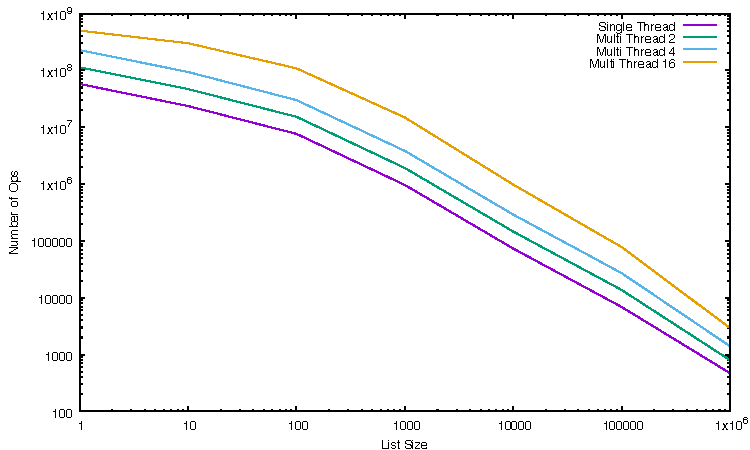
\includegraphics[height=2in]{outputData/baseline.pdf}
		\label{f:Fig.1}
		\caption{baseline reads/sec by list size logscale}
	\end{figure}


\section{Big Mutex Lock}
	\begin{figure}[h]
		\centering
		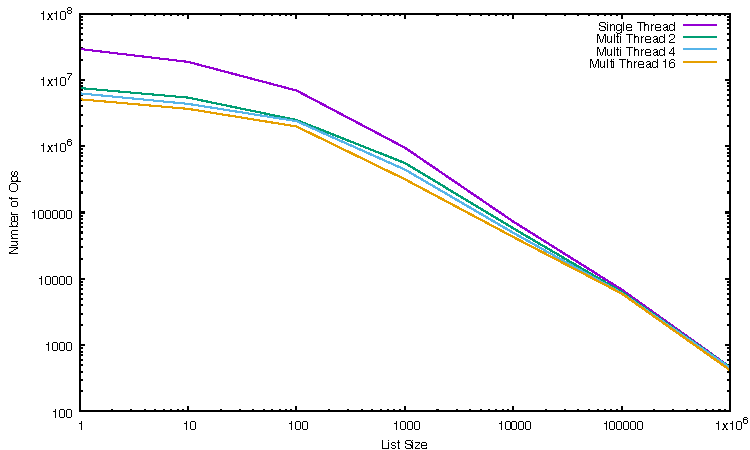
\includegraphics[height=2in]{outputData/bfl_mutex.pdf}
		\label{f:Fig.2}
		\caption{Mutex Lock ops/sec by list size logscale}
	\end{figure}
The program tested in \ref{f:Fig.2} is implemented by placing a mutex lock on the head of 
the linked list and locking the entire list for the duration of the operation. 
\newline
\newline
The performance of the single threaded instance of the Mutex lock underperforms the 
baseline by a factor of 2. The atomic operations to obtain and release the lock overcome 
the time to access for small lists. As the list approaches size of 1e6 the time converges 
with the baseline. 
\newline
\newline
The performance of the multi threaded instances over the baseline performs worse. For 
the 2 thread instance a 50x reduction for small lists and the 4 thread instance a 66x 
reduction. The mutex lock works by putting the threads to sleep while they wait for the 
lock to become available. The overhead of putting the threads to sleep overcomes the 
benefits of concurrency for small lists. As the list size grows we observe the threads
converging to the same number of ops / sec. The single lock forces the program to run 
more or less sequentially. As the time to perform an operation increases with list size 
the difference in overhead time becomes proportionately smaller. 


\section{Mutex v Spinlock on Single Core}
	\begin{figure}[h]
		\centering
		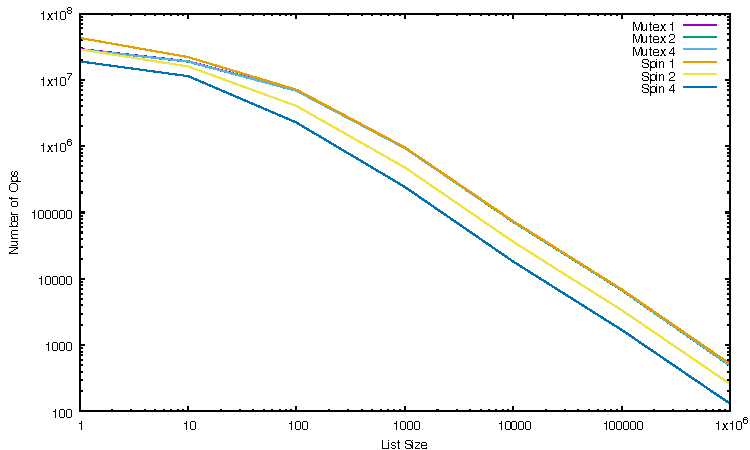
\includegraphics[height=2in]{outputData/bfl_spin_v_mutex.pdf}
		\label{f:Fig.3}
		\caption{Mutex and Spin Lock ops/sec on single core logscale}
	\end{figure}
\ref{f:Fig.3} shows the single threaded spinlock outperforming the mutex lock for small 
lists with all the concurrent mutex lock performances converging with the single threaded 
spinlock instance for large lists. This observation corresponds with that of concurrency 
in section 3. 
\newline
\newline
Its also observed that the 4-thread spinlock performs about half as many operations as 
the single threaded version and the 2-thread spinlock performs about 3/4 the operations of 
the single threaded version. This is a result of context switching. When one thread holds 
the lock it is taken out of scope by the scheduler and the alternate thread will spin on 
the processor waiting for a lock that will not be released by a sleeping thread. 

\section{Readers Writer Lock}
	\begin{figure}[h]
		\centering
		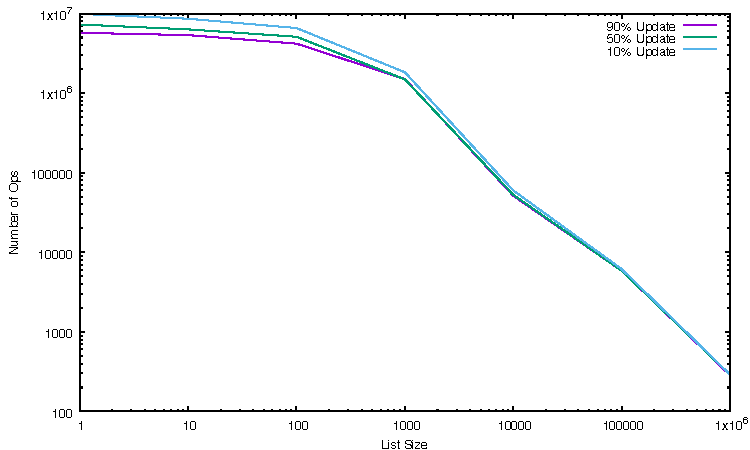
\includegraphics[height=2in]{outputData/bfl_rw.pdf}
		\label{f:Fig.4}
		\caption{Reader-Writer Lock ops/sec}
	\end{figure}
The readers-write lock defines a lock hierarchy where multiple reads can share a lock but 
writes cannot share with reads. \ref{f:Fig.4} shows that for small lists fewer writes yields 
more operations / sec. This is an expected observation because reads can access a lock 
concurrently but writes cannot. In reference to \ref{f:Fig.2} the readers 
writer lock performs as well as the single thread lock for small mutex lists and converges 
at the same time / op for large lists. For small to medium sized lists the readers writer 
lock is a good option when the number of reads is expected to outnumber the number of 
writes.  

\section{Hand over Hand Nodewise Lock}
	\begin{figure}[h]
		\centering
		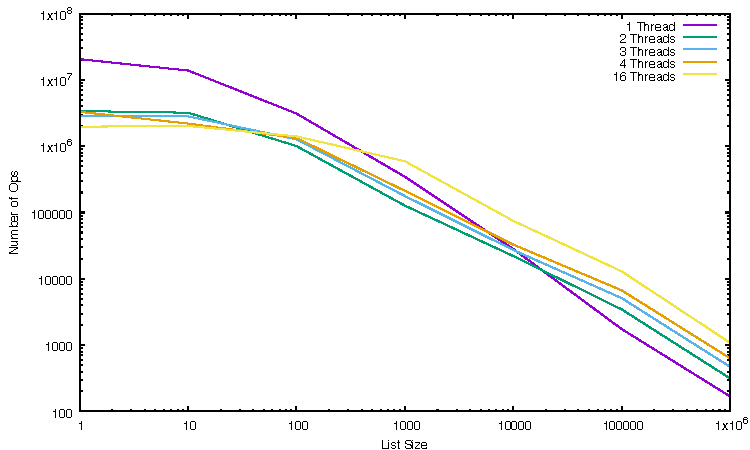
\includegraphics[height=2in]{outputData/hhl.pdf}
		\label{f:Fig.5}
		\caption{Spinlock on individual linked list nodes ops/sec logscale}
	\end{figure}
Observations from \ref{f:Fig.5} show that for a large number of threads, the Hand over 
Hand lock does performs better on large lists than the big Mutex lock in \ref{f:Fig.2}. 
This is because the HHL method allows multiple threads to work on the list at the same 
time, as long as the read or insert occurs earlier in the list than the latest lock. 
This allows for some concurrency vs the bfl implementation which bottlenecks the threads 
at the front of the list. 


\end{document}
